% ============================================================
%  article.tex -- Multi-Agent Systems & Autonomous AI
%  Main language: Hebrew   Secondary language: English
%  Compiler: XeLaTeX
% ============================================================

% -- 1. fontspec (must precede polyglossia) -------------------
\documentclass[12pt,a4paper]{article}

\usepackage{fontspec}
\setmainfont{Times New Roman}
\setsansfont{Arial}
\setmonofont{Courier New}

% -- 2. polyglossia -------------------------------------------
\usepackage{polyglossia}
\setmainlanguage{english}
\setotherlanguage{hebrew}

% -- 3. geometry ----------------------------------------------
\usepackage[
  a4paper,
  top=2.5cm, bottom=2.5cm,
  left=2.5cm, right=2.5cm,
  headheight=15pt
]{geometry}

% -- 4. fancyhdr ----------------------------------------------
\usepackage{fancyhdr}
\pagestyle{fancy}
\fancyhf{}
\fancyhead[R]{\small \begin{english}Multi-Agent Systems \& Autonomous AI\end{english}}
\fancyhead[L]{\small \thepage}
\fancyfoot[C]{\small \textit{\begin{english}MAS -- Comprehensive Review\end{english}}}
\renewcommand{\headrulewidth}{0.4pt}
\renewcommand{\footrulewidth}{0.4pt}

% -- 5. graphicx ----------------------------------------------
\usepackage{graphicx}

% -- 6. amsmath + amssymb -------------------------------------
\usepackage{amsmath}
\usepackage{amssymb}

% -- 7. booktabs + tabularx -----------------------------------
\usepackage{booktabs}
\usepackage{tabularx}

% -- 8. tikz --------------------------------------------------
\usepackage{tikz}
\usetikzlibrary{shapes.geometric,arrows.meta,positioning,fit,backgrounds}

% -- 9. biblatex ----------------------------------------------
\usepackage[
  backend=biber,
  style=authoryear,
  sorting=nyt,
  maxbibnames=5
]{biblatex}
\addbibresource{references.bib}

% -- 10. hyperref ---------------------------------------------
\usepackage[
  colorlinks=true,
  linkcolor=blue!70!black,
  citecolor=green!50!black,
  urlcolor=blue!60!black
]{hyperref}

% -- 11. bidi (MUST be last) ----------------------------------
\usepackage{bidi}

% -- Utility macros -------------------------------------------
\newcommand{\term}[1]{\LR{\textit{#1}}}
\newcommand{\fw}[1]{\LR{\texttt{#1}}}

% -- Inline bibliography via filecontents ---------------------
\usepackage{filecontents}
\begin{filecontents}{references.bib}
@article{wooldridge1995intelligent,
  author  = {Wooldridge, Michael and Jennings, Nicholas R.},
  title   = {Intelligent Agents: Theory and Practice},
  journal = {The Knowledge Engineering Review},
  year    = {1995},
  volume  = {10},
  number  = {2},
  pages   = {115--152}
}
@book{russell2020artificial,
  author    = {Russell, Stuart and Norvig, Peter},
  title     = {Artificial Intelligence: A Modern Approach},
  edition   = {4},
  publisher = {Pearson},
  year      = {2020}
}
@article{lowe2017multiagent,
  author  = {Lowe, Ryan and Wu, Yi and Tamar, Aviv and Harb, Jean and
             Abbeel, Pieter and Mordatch, Igor},
  title   = {Multi-Agent Actor-Critic for Mixed Cooperative-Competitive Environments},
  journal = {Advances in Neural Information Processing Systems},
  year    = {2017},
  volume  = {30}
}
@inproceedings{vinyals2019grandmaster,
  author    = {Vinyals, Oriol and Babuschkin, Igor and Czarnecki, Wojciech M. and others},
  title     = {Grandmaster Level in {StarCraft II} Using Multi-Agent Reinforcement Learning},
  booktitle = {Nature},
  year      = {2019},
  volume    = {575},
  pages     = {350--354}
}
@article{wang2024survey,
  author  = {Wang, Lei and Ma, Chen and Feng, Xueyang and others},
  title   = {A Survey on Large Language Model Based Autonomous Agents},
  journal = {Frontiers of Computer Science},
  year    = {2024},
  volume  = {18},
  number  = {6},
  pages   = {186345}
}
@misc{autogen2023,
  author       = {Wu, Qingyun and Bansal, Gagan and Zhang, Jieyu and others},
  title        = {{AutoGen}: Enabling Next-Gen {LLM} Applications via Multi-Agent Conversation},
  year         = {2023},
  howpublished = {arXiv:2308.08155}
}
@misc{crewai2024,
  author       = {Moura, Joao},
  title        = {{CrewAI}: Framework for Orchestrating Role-Playing Autonomous {AI} Agents},
  year         = {2024},
  howpublished = {\url{https://github.com/joaomdmoura/crewai}}
}
@misc{langgraph2024,
  author       = {Chase, Harrison and others},
  title        = {{LangGraph}: Building Stateful, Multi-Actor Applications with {LLM}s},
  year         = {2024},
  howpublished = {\url{https://github.com/langchain-ai/langgraph}}
}
@misc{llamaindex2024,
  author       = {Liu, Jerry and others},
  title        = {{LlamaIndex}: Data Framework for {LLM} Applications},
  year         = {2024},
  howpublished = {\url{https://github.com/run-llama/llama_index}}
}
@misc{mcp2024,
  author       = {{Anthropic}},
  title        = {Model Context Protocol ({MCP})},
  year         = {2024},
  howpublished = {\url{https://modelcontextprotocol.io}}
}
@misc{a2a2024,
  author       = {{Google DeepMind}},
  title        = {Agent-to-Agent ({A2A}) Communication Protocol},
  year         = {2024},
  howpublished = {\url{https://deepmind.google}}
}
@article{dafoe2020open,
  author  = {Dafoe, Allan},
  title   = {Open Problems in Cooperative {AI}},
  journal = {arXiv preprint arXiv:2012.08630},
  year    = {2020}
}
@techreport{marketusMAS2024,
  author      = {{Market.us}},
  title       = {Multi-Agent Systems Market Report 2024--2034},
  institution = {Market.us Research},
  year        = {2024}
}
@article{fipa1997,
  author  = {{FIPA -- Foundation for Intelligent Physical Agents}},
  title   = {{FIPA} Agent Communication Language Specifications},
  journal = {FIPA Technical Report},
  year    = {1997}
}
@article{labrou1997kqml,
  author  = {Labrou, Yannis and Finin, Tim},
  title   = {A Proposal for a New {KQML} Specification},
  journal = {Technical Report CS-97-03, University of Maryland Baltimore County},
  year    = {1997}
}
@article{galileo2024hallucination,
  author  = {{Galileo AI}},
  title   = {Hallucination Index: Evaluating {LLM} Reliability},
  journal = {Galileo AI Technical Report},
  year    = {2024}
}
@article{ibm2024enterprise,
  author  = {{IBM Institute for Business Value}},
  title   = {Enterprise {AI} Automation Outlook 2024},
  journal = {IBM Research Report},
  year    = {2024}
}
\end{filecontents}

% =============================================================
\begin{document}

% =============================================================
%  TITLE PAGE
% =============================================================
\begin{titlepage}
  \centering
  \vspace*{2cm}

  {\Huge\bfseries
   \begin{hebrew}
   \RL{%
   \texthebrew{%
   \char"05DE\char"05E2\char"05E8\char"05DB\char"05D5\char"05EA%
   \ %
   \char"05E8\char"05D1-%
   \char"05E1\char"05D5\char"05DB\char"05E0\char"05D9\char"05D5\char"05EA%
   \ %
   \char"05D5\char"05D1\char"05D9\char"05E0\char"05D4%
   \ %
   \char"05DE\char"05DC\char"05D0\char"05DB\char"05D5\char"05EA\char"05D9\char"05EA%
   \ %
   \char"05D0\char"05D5\char"05D8\char"05D5\char"05E0\char"05D5\char"05DE\char"05D9\char"05EA%
   }%
   }
   \end{hebrew}%
  }

  \vspace{0.5cm}
  {\large\bfseries
   \begin{english}Multi-Agent Systems (MAS) \& Autonomous AI\end{english}}

  \vspace{1.5cm}
  \rule{0.8\textwidth}{1pt}

  \vspace{1cm}
  {\large
   \begin{english}A Comprehensive Review: Architectures, Learning, Frameworks \& Safety\end{english}}

  \vspace{2cm}

  \begin{tikzpicture}
    \node[draw=blue!70!black, fill=blue!5, rounded corners=8pt,
          minimum width=9cm, minimum height=2.5cm, text width=8.5cm,
          align=center] {
      \begin{english}
      {\bfseries Key Topics}\\[6pt]
      Agent Architectures $\cdot$ Multi-Agent RL\\
      Communication Protocols $\cdot$ LLM Frameworks\\
      Real-World Applications $\cdot$ Safety \& Alignment
      \end{english}
    };
  \end{tikzpicture}

  \vfill

  {\normalsize
   \begin{english}
   Sources: Market.us 2024 $\cdot$ arXiv 2024--2025 $\cdot$
   DeepMind $\cdot$ Cooperative AI Foundation $\cdot$ IBM $\cdot$ Galileo AI
   \end{english}}

  \vspace{0.5cm}
  {\normalsize \LR{\today}}

  \vspace{0.4cm}
  \begin{english}
  \begin{tabular}{rl}
    \textbf{Author:}   & [Your Name] \\
    \textbf{Course:}   & AI Agents --- MSC Course, HW3 \\
    \textbf{Lecturer:} & Dr.\ Yoram Segal \\
  \end{tabular}
  \end{english}
\end{titlepage}

% =============================================================
%  TABLE OF CONTENTS
% =============================================================
\tableofcontents
\newpage

% =============================================================
%  ABSTRACT
% =============================================================
\begin{abstract}
\begin{english}
Multi-Agent Systems (MAS) represent a central paradigm in modern artificial
intelligence, in which multiple autonomous agents operate in a shared environment,
coordinate with each other, and achieve goals that cannot be accomplished by a
single agent. With the rise of Large Language Models (LLMs), new possibilities
have opened for inter-agent coordination, autonomous planning, and execution of
complex tasks. This article surveys the broad landscape of MAS: from foundational
concepts to contemporary frameworks, with emphasis on safety, alignment, and
reliability challenges. The global MAS market is projected to grow from \$15B
in 2024 to approximately \$375B in 2034, representing a compound annual growth
rate of approximately 48.6\% \autocite{marketusMAS2024}.
\end{english}
\end{abstract}

\newpage

% =============================================================
%  SECTION 1 -- INTRODUCTION
% =============================================================
\section{\begin{english}Introduction: The World of Autonomous Agents\end{english}}

\subsection{\begin{english}What is an Autonomous Agent?\end{english}}

\begin{english}
An autonomous agent is a computational entity that operates in an environment,
perceives it through sensors, and influences it through actuators.
According to \textcite{wooldridge1995intelligent}, an agent must possess four
core properties:
\end{english}

\begin{enumerate}
  \item \begin{english}\textbf{Autonomy} --- acting without constant direct human intervention.\end{english}
  \item \begin{english}\textbf{Sociability} --- ability to communicate with other agents.\end{english}
  \item \begin{english}\textbf{Reactivity} --- perceiving and responding to environmental changes.\end{english}
  \item \begin{english}\textbf{Proactiveness} --- taking goal-directed initiative.\end{english}
\end{enumerate}

\subsection{\begin{english}Agent Architectures: Historical Evolution\end{english}}

\begin{english}
The evolution of agent architectures spans five major stages, illustrated in the
visualisation dashboard (see Section~\ref{sec:visualization}):
\end{english}

\begin{description}
  \item[\begin{english}1980--1995\end{english}]
        \begin{english}\textbf{Simple Rule-Based Agents} --- rigid \term{if-then} logic with no learning capability.\end{english}
  \item[\begin{english}1995--2005\end{english}]
        \begin{english}\textbf{Model-Based Agents} --- internal representation of world state.\end{english}
  \item[\begin{english}2005--2015\end{english}]
        \begin{english}\textbf{Goal \& Utility Agents} --- optimisation of utility functions.\end{english}
  \item[\begin{english}2015--2020\end{english}]
        \begin{english}\textbf{Learning Agents} --- Reinforcement Learning (\term{RL}).\end{english}
  \item[\begin{english}2020--Present\end{english}]
        \begin{english}\textbf{LLM-Powered Agents} --- planning, reasoning, and linguistic coordination.\end{english}
\end{description}

\subsection{\begin{english}MAS Architectures: A Comparison\end{english}}

\begin{english}
Multi-agent systems can be classified by their organisational structure
\autocite{russell2020artificial}:
\end{english}

\begin{description}
  \item[\term{Hierarchical}]
        \begin{english}Hierarchical structure with an orchestrator agent and sub-agents.
        Enables simple coordination but may create bottlenecks.\end{english}
  \item[\term{Peer-to-Peer}]
        \begin{english}All agents are equal; decentralised coordination.
        More fault-tolerant but harder to manage.\end{english}
  \item[\term{Hybrid}]
        \begin{english}Combines both approaches: hierarchical management at the high level
        and peer-to-peer coordination at the low level.\end{english}
\end{description}

\subsection{\begin{english}Key Formulae in MAS Theory\end{english}}

\subsubsection{\begin{english}Utility Function and Reward\end{english}}

\begin{english}
In the formal definition of a rational agent, the agent seeks the action that
maximises expected utility:
\end{english}

\begin{english}
\begin{equation}
  \pi^{*}(s) = \arg\max_{a \in \mathcal{A}} \mathbb{E}\!\left[
    \sum_{t=0}^{\infty} \gamma^{t} r_{t+1}
    \;\middle|\; s_0 = s,\; \pi
  \right]
  \label{eq:optimal_policy}
\end{equation}
\end{english}

\begin{english}
where $\pi^{*}$ is the optimal policy, $\gamma \in [0,1)$ is the discount factor,
$r_{t}$ is the reward at step $t$, and $\mathcal{A}$ is the action space.
\end{english}

\subsubsection{\begin{english}Bellman Equation for a Multi-Agent Environment\end{english}}

\begin{english}
In an environment with $n$ agents, the joint state value is defined by:
\end{english}

\begin{english}
\begin{equation}
  V^{\boldsymbol{\pi}}(\mathbf{s}) = \sum_{i=1}^{n}
  \mathbb{E}_{\boldsymbol{\pi}}\!\left[
    \sum_{t=0}^{\infty} \gamma^{t} r^{(i)}_{t}
    \;\middle|\; \mathbf{s}_0 = \mathbf{s}
  \right]
  \label{eq:bellman_mas}
\end{equation}
\end{english}

\begin{english}
where $\mathbf{s} = (s^{(1)}, s^{(2)}, \ldots, s^{(n)})$ is the joint system state
and $r^{(i)}_{t}$ is the reward of agent $i$ at step $t$.
\end{english}

\subsubsection{\begin{english}MAS Market CAGR Model\end{english}}

\begin{english}
The MAS market forecast relies on the Compound Annual Growth Rate (CAGR) model:
\end{english}

\begin{english}
\begin{equation}
  V(t) = V_0 \cdot (1 + r)^{t}
  \label{eq:cagr}
\end{equation}
\end{english}

\begin{english}
where $V_0 = \$15\text{B}$ (2024 baseline), $r = 0.486$ (CAGR of 48.6\%),
and $t$ is the number of years from 2024. At $t = 10$ (year 2034):
\end{english}

\begin{english}
\begin{align}
  V(10) &= 15 \cdot (1.486)^{10} \notag \\
        &\approx 15 \cdot 25.0    \notag \\
        &\approx \$375\text{B}
  \label{eq:market_forecast}
\end{align}
\end{english}

\subsection{\begin{english}Formal Definition of MAS\end{english}}

\begin{english}
A Multi-Agent System can be formally defined as a tuple:
\begin{equation}
  \mathcal{M} = \langle
    \mathcal{I},\;
    \mathcal{E},\;
    \{A_i\}_{i \in \mathcal{I}},\;
    \{\Omega_i\}_{i \in \mathcal{I}},\;
    \mathcal{T},\;
    \{R_i\}_{i \in \mathcal{I}}
  \rangle
  \label{eq:mas_formal}
\end{equation}
where $\mathcal{I} = \{1, 2, \ldots, n\}$ is the set of agents, $\mathcal{E}$ is
the shared environment, $A_i$ is the action space of agent $i$, $\Omega_i$ is the
observation space, $\mathcal{T}$ is the joint transition function, and $R_i$ is
the reward function of agent $i$.
\end{english}

\subsection{\begin{english}Market Forecast\end{english}}

\begin{english}
The global MAS market is in rapid growth. According to \textcite{marketusMAS2024},
it is expected to surpass the \$375B threshold by 2034. Key growth drivers include:
\end{english}

\begin{itemize}
  \item \begin{english}\textbf{LLM Maturity}: improvements in reasoning, memory, and tool-calling capabilities.\end{english}
  \item \begin{english}\textbf{Enterprise Demand}: automation of complex business processes \autocite{ibm2024enterprise}.\end{english}
  \item \begin{english}\textbf{Academic Research}: sharp rise in arXiv publications on autonomous agents.\end{english}
  \item \begin{english}\textbf{Cloud Infrastructure}: low-cost compute availability for multi-agent deployments.\end{english}
\end{itemize}

% =============================================================
%  SECTION 2 -- COMMUNICATION PROTOCOLS
% =============================================================
\section{\begin{english}Agent Communication Protocols\end{english}}

\subsection{\begin{english}Historical Background\end{english}}

\begin{english}
Inter-agent communication is one of the central challenges in MAS.
The first protocols were developed in the 1990s:
\end{english}

\subsubsection{\begin{english}KQML (1993--1999)\end{english}}

\begin{english}
\term{Knowledge Query and Manipulation Language} (KQML) was one of the first
protocols for inter-agent communication \autocite{labrou1997kqml}. It defined a
set of \term{performatives} --- speech acts such as \fw{TELL}, \fw{ASK},
and \fw{SUBSCRIBE}.
\end{english}

\subsubsection{\begin{english}FIPA (1997--2005)\end{english}}

\begin{english}
\term{Foundation for Intelligent Physical Agents} (FIPA) developed more
comprehensive standards \autocite{fipa1997}, including an Agent Communication
Language (ACL) and interaction protocols.
\end{english}

\subsection{\begin{english}Contemporary Protocols: The LLM Era\end{english}}

\subsubsection{\begin{english}Model Context Protocol (MCP)\end{english}}

\begin{english}
Anthropic's MCP \autocite{mcp2024} defines a unified interface between LLM agents
and tools / data sources. The protocol is based on JSON-RPC and enables:
\end{english}

\begin{itemize}
  \item \begin{english}Access to external tools\end{english}
  \item \begin{english}Resource reading\end{english}
  \item \begin{english}Structured prompt usage\end{english}
\end{itemize}

\subsubsection{\begin{english}Agent-to-Agent (A2A) by Google\end{english}}

\begin{english}
Google DeepMind's A2A protocol \autocite{a2a2024} focuses on direct agent-to-agent
communication, defining \term{Agent Cards} --- standardised capability descriptors.
\end{english}

\subsubsection{\begin{english}Agent Communication Protocol (ACP)\end{english}}

\begin{english}
ACP (2024) is an open protocol based on REST API, designed to enable asynchronous
communication between agents in production environments.
\end{english}

% =============================================================
%  SECTION 3 -- MARL
% =============================================================
\section{\begin{english}Multi-Agent Reinforcement Learning (MARL)\end{english}}

\subsection{\begin{english}Introduction to MARL\end{english}}

\begin{english}
Multi-Agent Reinforcement Learning (MARL) extends the classical RL framework to
environments with multiple simultaneously learning agents \autocite{lowe2017multiagent}.
The central challenge is \textbf{non-stationarity}: as all agents learn
simultaneously, the environment becomes dynamic from each agent's perspective.
\end{english}

\subsection{\begin{english}MARL Frameworks\end{english}}

\subsubsection{\begin{english}Fully Cooperative\end{english}}

\begin{english}
All agents share a common reward function:
\end{english}

\begin{english}
\begin{equation}
  R_{\text{cooperative}} = \frac{1}{n} \sum_{i=1}^{n} r^{(i)}
  \label{eq:cooperative_reward}
\end{equation}
\end{english}

\subsubsection{\begin{english}Fully Competitive (Zero-Sum)\end{english}}

\begin{english}
\begin{equation}
  \sum_{i=1}^{n} r^{(i)} = 0 \quad \forall\, t
  \label{eq:zero_sum}
\end{equation}
\end{english}

\subsubsection{\begin{english}Mixed Setting\end{english}}

\begin{english}
Most real-world environments are mixed --- cooperation within groups and competition
between groups.
\end{english}

\subsection{\begin{english}Emergent Behaviour\end{english}}

\begin{english}
One of the most fascinating phenomena in MARL is the emergence of complex strategies
that were not explicitly programmed. \textcite{vinyals2019grandmaster} demonstrated
this in StarCraft~II, where agents developed sophisticated military tactics.
The emergence threshold can be quantified by a sigmoid model:
\end{english}

\begin{english}
\begin{equation}
  C(t) = \frac{1}{1 + e^{-k(t - t_0)}} \cdot C_{\max}
  \label{eq:emergence_sigmoid}
\end{equation}
\end{english}

\begin{english}
where $C(t)$ is the cooperation metric at step $t$, $k$ is the learning rate,
$t_0$ is the emergence threshold, and $C_{\max}$ is the maximum value.
\end{english}

% =============================================================
%  SECTION 4 -- LLM FRAMEWORKS
% =============================================================
\section{\begin{english}LLM-Powered Agent Frameworks\end{english}}

\subsection{\begin{english}Introduction\end{english}}

\begin{english}
The rise of LLMs such as GPT-4, Claude, and Gemini has created a new wave of
frameworks for building multi-agent systems \autocite{wang2024survey}. These
frameworks leverage the reasoning, planning, and tool-use capabilities of LLMs.
\end{english}

\subsection{\begin{english}AutoGen (Microsoft)\end{english}}

\begin{english}
\fw{AutoGen} \autocite{autogen2023} is a framework from Microsoft Research enabling
multi-agent conversational workflows. Key features:
\end{english}

\begin{itemize}
  \item \begin{english}\textbf{Conversational Interface}: agents communicate via natural-language messages.\end{english}
  \item \begin{english}\textbf{Code Execution}: built-in support for Python and Bash execution.\end{english}
  \item \begin{english}\textbf{Flexibility}: supports a wide range of LLMs (commercial and open-source).\end{english}
  \item \begin{english}\textbf{Research}: particularly suited for academic experimentation.\end{english}
\end{itemize}

\subsection{\begin{english}CrewAI\end{english}}

\begin{english}
\fw{CrewAI} \autocite{crewai2024} introduces the paradigm of \textbf{role-based agent teams}.
Each agent is defined with:
\end{english}

\begin{itemize}
  \item \begin{english}\textbf{Role}: definition of what the agent does.\end{english}
  \item \begin{english}\textbf{Goal}: what the agent aims to achieve.\end{english}
  \item \begin{english}\textbf{Backstory}: context and personality.\end{english}
  \item \begin{english}\textbf{Tools}: external capabilities.\end{english}
\end{itemize}

\subsection{\begin{english}LangGraph\end{english}}

\begin{english}
\fw{LangGraph} \autocite{langgraph2024} represents a graph-based approach to agent
coordination. The graph is defined as a DAG (Directed Acyclic Graph) or a cyclic
graph with control mechanisms. Well-suited for production environments requiring
high reliability.
\end{english}

\subsection{\begin{english}LlamaIndex\end{english}}

\begin{english}
\fw{LlamaIndex} \autocite{llamaindex2024} specialises in integrating LLMs with
external data sources via Retrieval-Augmented Generation (RAG).
\end{english}

\subsection{\begin{english}Framework Comparison Table\end{english}}

\begin{table}[ht]
  \centering
  \caption{\begin{english}Comparison of LLM-Powered MAS Frameworks\end{english}}
  \label{tab:frameworks}
  \begin{english}
  \begin{tabularx}{\textwidth}{lXXXX}
    \toprule
    \textbf{Criterion} & \textbf{AutoGen} & \textbf{CrewAI} & \textbf{LangGraph} & \textbf{LlamaIndex} \\
    \midrule
    Ease of Use           & High (4/5)      & Very High (5/5) & Low (2/5)       & Medium (3/5)    \\
    Production Readiness  & Medium (3/5)    & High (4/5)      & Very High (5/5) & High (4/5)      \\
    Flexibility           & High (4/5)      & Medium (3/5)    & Very High (5/5) & High (4/5)      \\
    Research Suitability  & Very High (5/5) & Medium (3/5)    & Medium (3/5)    & High (4/5)      \\
    Primary Paradigm      & Conversational  & Role-based Teams & Graph-based    & RAG / Data      \\
    \bottomrule
  \end{tabularx}
  \end{english}
  \vspace{4pt}
  {\small \begin{english}Source: author analysis based on \autocite{autogen2023,crewai2024,langgraph2024,llamaindex2024}\end{english}}
\end{table}

% =============================================================
%  SECTION 5 -- REAL-WORLD APPLICATIONS
% =============================================================
\section{\begin{english}Real-World Applications\end{english}}

\subsection{\begin{english}Healthcare\end{english}}

\begin{english}
MAS in medicine includes:
\end{english}

\begin{itemize}
  \item \begin{english}\textbf{Collaborative Diagnosis}: specialised agents across medical domains cooperate for diagnosis.\end{english}
  \item \begin{english}\textbf{Hospital Management}: optimisation of schedules, inventory, and resource allocation.\end{english}
  \item \begin{english}\textbf{Drug Discovery}: agents run large-scale \textit{in silico} experiments.\end{english}
\end{itemize}

\subsection{\begin{english}Finance\end{english}}

\begin{english}
In the financial domain, MAS are used for:
\end{english}

\begin{itemize}
  \item \begin{english}\textbf{Algorithmic Trading}: agents manage investment portfolios and react to market signals.\end{english}
  \item \begin{english}\textbf{Fraud Detection}: agent networks analyse transactions in real time.\end{english}
  \item \begin{english}\textbf{Risk Management}: systemic risk assessment across complex portfolios.\end{english}
\end{itemize}

\subsection{\begin{english}Robotics and Autonomous Vehicles\end{english}}

\begin{itemize}
  \item \begin{english}\textbf{Robot Swarms}: robotic agents coordinate for logistics tasks.\end{english}
  \item \begin{english}\textbf{Autonomous Vehicles}: inter-vehicle coordination for collision avoidance and traffic optimisation.\end{english}
  \item \begin{english}\textbf{Space Exploration}: robotic agents for exploring hazardous environments.\end{english}
\end{itemize}

\subsection{\begin{english}Enterprise Automation\end{english}}

\begin{english}
\textcite{ibm2024enterprise} report that MAS-based enterprise automation shows
the highest adoption index (90\%) among all domains.
\end{english}

\subsection{\begin{english}Application Domains Table\end{english}}

\begin{table}[ht]
  \centering
  \caption{\begin{english}MAS Application Domains --- Adoption and Safety Requirement Indices\end{english}}
  \label{tab:domains}
  \begin{english}
  \begin{tabularx}{\textwidth}{lXcc}
    \toprule
    \textbf{Domain} & \textbf{Key Use Cases} & \textbf{Adoption (\%)} & \textbf{Safety Req. (\%)} \\
    \midrule
    Healthcare            & Diagnosis, drug discovery, scheduling       & 72 & 88 \\
    Finance               & Algorithmic trading, fraud detection        & 85 & 75 \\
    Robotics              & Swarm coordination, logistics               & 68 & 82 \\
    Autonomous Vehicles   & Traffic optimisation, collision avoidance   & 60 & 95 \\
    Enterprise Automation & Workflow, RPA, customer service             & 90 & 65 \\
    Smart Grid / IoT      & Energy balancing, predictive maintenance    & 55 & 70 \\
    \bottomrule
  \end{tabularx}
  \end{english}
  \vspace{4pt}
  {\small \begin{english}Source: \autocite{marketusMAS2024,ibm2024enterprise}\end{english}}
\end{table}

% =============================================================
%  SECTION 6 -- SAFETY & ALIGNMENT
% =============================================================
\section{\begin{english}Safety, Alignment, and Reliability\end{english}}

\subsection{\begin{english}Safety Challenges in MAS\end{english}}

\begin{english}
When multiple autonomous agents operate together, unique safety challenges arise
\autocite{dafoe2020open}:
\end{english}

\subsubsection{\begin{english}Miscoordination\end{english}}

\begin{english}
Coordination failure between agents can lead to conflicting decisions, such as two
robots simultaneously attempting to grasp the same object. According to
\textcite{dafoe2020open}, this is the most common failure mode (28\% of cases).
\end{english}

\subsubsection{\begin{english}Conflict\end{english}}

\begin{english}
Agents with opposing goals may enter deadlock or cause damage. Frequency: 22\%.
\end{english}

\subsubsection{\begin{english}Collusion\end{english}}

\begin{english}
In competitive environments, agents may develop unintended collusion strategies.
Frequency: 18\%.
\end{english}

\subsubsection{\begin{english}Hallucination Propagation\end{english}}

\begin{english}
When one LLM agent generates incorrect information, it may propagate to other
agents in the system \autocite{galileo2024hallucination}. Frequency: 20\%.
\end{english}

\subsubsection{\begin{english}Context Overflow\end{english}}

\begin{english}
In long conversations, agents may lose critical information. Frequency: 12\%.
\end{english}

\subsection{\begin{english}Cooperative AI Principles\end{english}}

\begin{english}
\textcite{dafoe2020open} proposes a framework for Cooperative AI development
comprising:
\end{english}

\begin{enumerate}
  \item \begin{english}\textbf{Understanding}: agents understand the goals and constraints of other agents.\end{english}
  \item \begin{english}\textbf{Communication}: reliable and transparent communication channels.\end{english}
  \item \begin{english}\textbf{Commitment}: ability to commit to future actions.\end{english}
  \item \begin{english}\textbf{Norms}: agreement on shared behavioural rules.\end{english}
\end{enumerate}

\subsection{\begin{english}Formal Safety Metrics\end{english}}

\begin{english}
A systemic safety metric can be defined as:
\end{english}

\begin{english}
\begin{equation}
  S_{\text{system}} = 1 - \prod_{i=1}^{n} (1 - S_i)
  \label{eq:system_safety}
\end{equation}
\end{english}

\begin{english}
where $S_i \in [0,1]$ is the safety metric of agent $i$. For a system with
$n = 5$ agents each with $S_i = 0.9$:
\end{english}

\begin{english}
\begin{align}
  S_{\text{system}} &= 1 - (1 - 0.9)^{5} \notag \\
                    &= 1 - (0.1)^{5}       \notag \\
                    &= 1 - 0.00001         \notag \\
                    &= 0.99999
  \label{eq:safety_example}
\end{align}
\end{english}

% =============================================================
%  SECTION 7 -- VISUALIZATION
% =============================================================
\section{\begin{english}Visualisation: MAS Metrics and Landscape\end{english}}
\label{sec:visualization}

\begin{english}
The dashboard below presents eight visual panels covering the central dimensions
of this subject. It was created using Matplotlib and NumPy, based on data from
\autocite{marketusMAS2024,autogen2023,crewai2024,langgraph2024,dafoe2020open,galileo2024hallucination}.
\end{english}

\begin{figure}[ht]
  \centering
  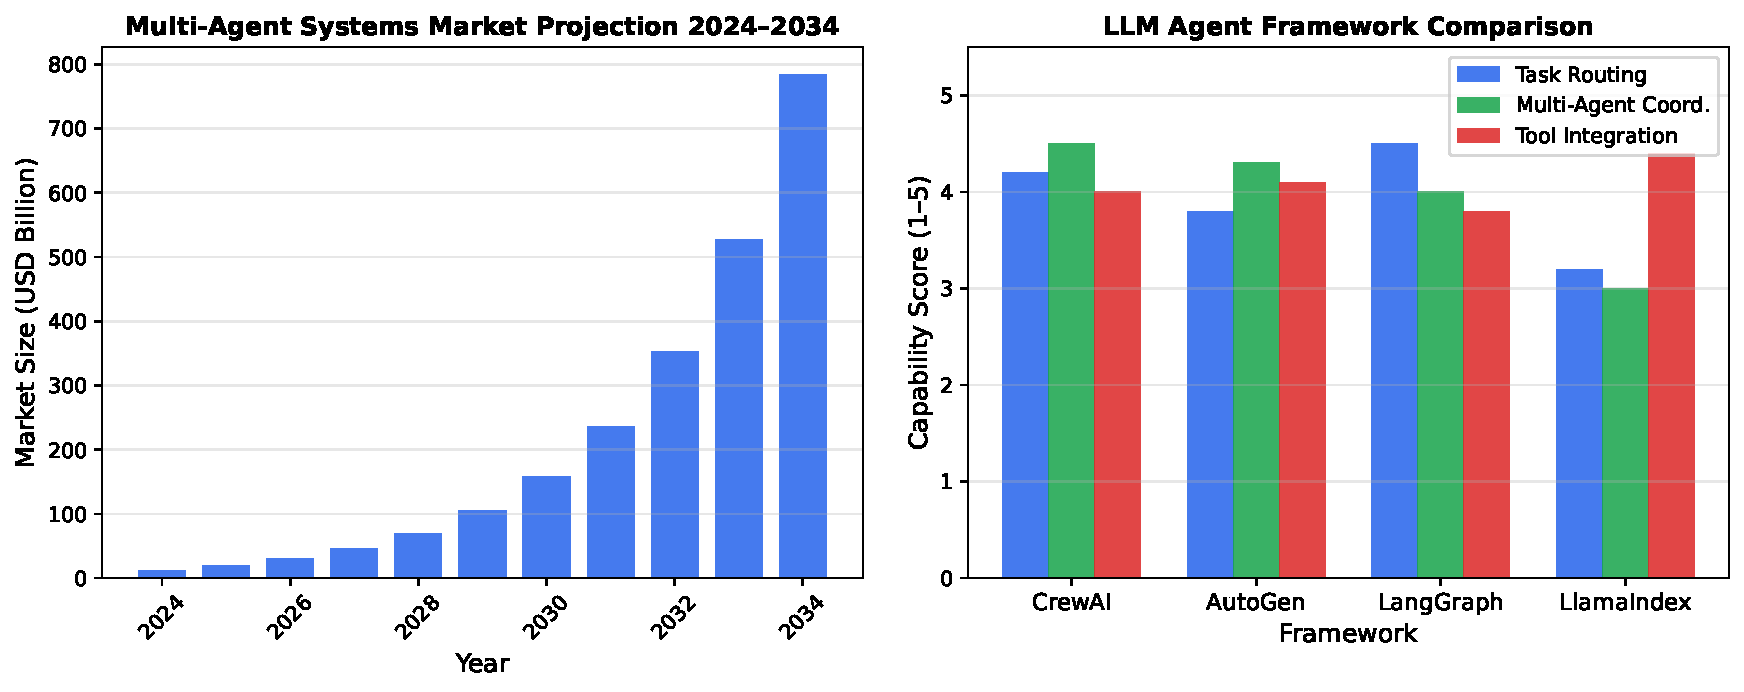
\includegraphics[width=\textwidth,keepaspectratio]{figures/graph.pdf}
  \caption{%
    \begin{english}
    Comprehensive dashboard: Multi-Agent Systems (MAS) \& Autonomous AI ---
    key metrics and market landscape.
    The 3$\times$3 dashboard covers:
    (1)~Global MAS market growth forecast (CAGR 48.6\%, Eq.~\ref{eq:cagr}),
    (2)~Agent architecture evolution timeline,
    (3)~MAS architecture radar comparison (Hierarchical vs.\ Peer-to-Peer vs.\ Hybrid),
    (4)~LLM-powered framework comparison (AutoGen / CrewAI / LangGraph / LlamaIndex),
    (5)~MARL emergent behaviour learning curves with emergence threshold
        (Eq.~\ref{eq:emergence_sigmoid}),
    (6)~Application domain adoption and safety requirement indices,
    (7)~Agent communication protocol timeline (KQML to ACP), and
    (8)~MAS safety risk distribution donut chart (five failure-mode categories).
    \end{english}%
  }
  \label{fig:dashboard}
\end{figure}

\subsection{\begin{english}Panel Interpretation\end{english}}

\begin{description}
  \item[\begin{english}Panel 1 --- MAS Market Growth\end{english}]
        \begin{english}Shows the growth forecast from \$15B in 2024 to \$375B in 2034,
        based on Equation~\ref{eq:cagr}.\end{english}

  \item[\begin{english}Panel 2 --- Historical Evolution\end{english}]
        \begin{english}Illustrates the five development stages of agent architectures,
        from rule-based agents to LLM-powered agents.\end{english}

  \item[\begin{english}Panel 3 --- Architecture Comparison\end{english}]
        \begin{english}Radar chart comparing Hierarchical, Peer-to-Peer, and Hybrid
        architectures across five dimensions.\end{english}

  \item[\begin{english}Panel 4 --- Frameworks\end{english}]
        \begin{english}Grouped bars comparing AutoGen, CrewAI, LangGraph, and LlamaIndex.\end{english}

  \item[\begin{english}Panel 5 --- MARL\end{english}]
        \begin{english}Learning curves demonstrating the emergence of cooperation in a
        training environment, based on Equation~\ref{eq:emergence_sigmoid}.\end{english}

  \item[\begin{english}Panel 6 --- Domains\end{english}]
        \begin{english}Horizontal bars of adoption and safety requirement indices by sector.\end{english}

  \item[\begin{english}Panel 7 --- Protocols\end{english}]
        \begin{english}Timeline of communication protocols from KQML to ACP.\end{english}

  \item[\begin{english}Panel 8 --- Safety Risks\end{english}]
        \begin{english}Donut chart of five MAS failure-mode categories.\end{english}
\end{description}

% =============================================================
%  SECTION 8 -- FUTURE DIRECTIONS
% =============================================================
\section{\begin{english}Future Directions and Open Challenges\end{english}}

\subsection{\begin{english}Technical Challenges\end{english}}

\begin{enumerate}
  \item \begin{english}\textbf{Scalability}: how to efficiently manage systems with thousands of agents?\end{english}
  \item \begin{english}\textbf{Fault Tolerance}: ensuring correct operation when some agents fail.\end{english}
  \item \begin{english}\textbf{Privacy}: preserving data privacy in distributed environments.\end{english}
  \item \begin{english}\textbf{Explainability}: understanding the decision-making processes of complex systems.\end{english}
\end{enumerate}

\subsection{\begin{english}Alignment and Governance Challenges\end{english}}

\begin{enumerate}
  \item \begin{english}\textbf{Value Alignment}: ensuring agent goals are consistent with human values \autocite{dafoe2020open}.\end{english}
  \item \begin{english}\textbf{Accountability}: who is responsible for the actions of an autonomous system?\end{english}
  \item \begin{english}\textbf{Regulation}: developing regulatory frameworks for MAS oversight.\end{english}
\end{enumerate}

\subsection{\begin{english}Emerging Research Trends\end{english}}

\begin{itemize}
  \item \begin{english}\textbf{Long-Term Memory Agents}: integration of vector databases for context retention.\end{english}
  \item \begin{english}\textbf{Hierarchical Planning}: agents planning at different levels of abstraction.\end{english}
  \item \begin{english}\textbf{Transfer Learning}: reusing knowledge acquired in one environment in another.\end{english}
  \item \begin{english}\textbf{Meta-Learning}: agents learning how to learn faster.\end{english}
\end{itemize}

% =============================================================
%  SECTION 9 -- CONCLUSION
% =============================================================
\section{\begin{english}Conclusion\end{english}}

\begin{english}
Multi-agent systems are undergoing a profound revolution with the rise of LLMs and
the development of sophisticated frameworks. This article has surveyed the broad
landscape:
\end{english}

\begin{itemize}
  \item \begin{english}\textbf{Architectures}: from simple agents to complex hybrid systems.\end{english}
  \item \begin{english}\textbf{Protocols}: from KQML and FIPA to MCP, A2A, and ACP.\end{english}
  \item \begin{english}\textbf{Learning}: MARL and emergent behaviour as the basis for collective intelligence.\end{english}
  \item \begin{english}\textbf{Frameworks}: AutoGen, CrewAI, LangGraph, and LlamaIndex.\end{english}
  \item \begin{english}\textbf{Applications}: from healthcare and finance to robotics and enterprise automation.\end{english}
  \item \begin{english}\textbf{Safety}: five failure-mode categories and Cooperative AI principles.\end{english}
\end{itemize}

\begin{english}
The MAS market is expected to grow 25-fold in the next decade. The success of this
revolution depends not only on technological development, but also on our ability
to build systems that are safe, reliable, and aligned with human values.
As \textcite{dafoe2020open} notes, cooperative artificial intelligence is not merely
a technical challenge but a profound societal one.
\end{english}

\begin{english}
The future of autonomous AI lies not in isolated intelligence, but in the emergent
wisdom of coordinated agent collectives --- systems that are greater than the sum of
their parts, yet remain aligned with human values and subject to meaningful oversight.
\end{english}

% =============================================================
%  BIBLIOGRAPHY
% =============================================================
\newpage
\printbibliography[title={\begin{english}Bibliography\end{english}}]

\end{document}
